\input{chapter-header.tex}
% ===========================================================================
\part{Bootstrapping: Explicit Application Runtime Generation}
% ===========================================================================
\chapter{Bootstrapping Object-Oriented Languages}
\chaplabel{bootstrapping}
\minitoc
\introduction
% ===========================================================================

The language initialization is the step during the execution of a program where the application and language runtime of such program is generated \ie the initial structures and constructs of a language runtime are set up.
As described in The Art of the Metaobject Protocol~(AMOP)~\cite{Kicz91a}, a language initialization solves the \emph{bootstrapping issues} of a language runtime. To achieve this the language initialization is often located in the virtual machine~(VM), where it can solve these issues without depending on running code on the language under construction.

\begin{figure}[ht!]
\begin{code}
void Init_class_hierarchy(void) {
    rb_cBasicObject = boot_defclass("BasicObject", 0);
    rb_cObject = boot_defclass("Object", rb_cBasicObject);
    rb_cModule = boot_defclass("Module", rb_cObject);
    rb_cClass =  boot_defclass("Class",  rb_cModule);

    rb_const_set(rb_cObject, rb_intern("BasicObject"),rb_cBasicObject);
    RBASIC_SET_CLASS(rb_cClass, rb_cClass);
    RBASIC_SET_CLASS(rb_cModule, rb_cClass);
    RBASIC_SET_CLASS(rb_cObject, rb_cClass);
    RBASIC_SET_CLASS(rb_cBasicObject, rb_cClass);
}
\end{code}
\caption{\textbf{Code of the Ruby \VM that initializes the class hierarchy (excerpt).} The \VM code fixes the language class hierarchy.\label{code:ruby_hierarchy}}
\end{figure}

For example, Figure \ref{code:ruby_hierarchy} shows an excerpt of the code that initializes the class hierarchy in the Ruby \VM written in C\footnote{Taken from the version 2.1 of the Ruby \VM in \url{http://svn.ruby-lang.org/repos/ruby}}. From this code, Ruby's basic class hierarchy is composed by \ct{BasicObject} as its root, followed by \ct{Object}, \ct{Module} and \ct{Class}. These classes are first created manually without instantiating any class, and once the class \ct{Class} is available, their class references are updated. As we stated in \chapref{state_modifying}, this has many negative consequences. First, the \VM~(the Ruby \VM in this case) fixes this basic class hierarchy and prevents us to change it without changing the \VM.
In addition, an unclear separation between the \VM and language concerns in the \VM code makes harder to change and adapt the language to other circumstances. Finally, when this \VM is written in a low-level language, we rely on the tools and abstractions this low-level language provides instead of the more powerful ones from the high-level language. 

%We developed a bootstrap process for an object-oriented language based on the following ideas: we introduce (a) the language definition as a self-description of the bootstrapped language~(a description of its elements and how to build itself, written in itself), (b) a \textbf{first-class runtime} that provides a clear \VM-language interface for its manipulation, and (c) a specialized code interpreter~(the \emph{bootstrapping interpreter}) that executes the language definition~(Figure \ref{fig:bootstrapping_overview}) to initialize the language runtime in the reified runtime through its clear \VM-language interface. These three explicit components allows the separation of concerns and decouple the initialization of the language runtime from the \VM initialization.

%Following those principles, we developed a bootstrap process for an object-oriented language with the following elements~(Figure \ref{fig:bootstrapping_overview}). These three explicit components decouple the initialization of the language runtime from the \VM initialization so we can define different languages on top of the same \VM. Additionally we can modify the language runtime using the abstractions and tools of the high-level language.

% at runtime, the \VM interpreter does not require this particular fixed class hierarchy nor the fact that classes have metaclasses. It is orthogonal.
%This unnecessary coupling has a double impact on the language infrastructure: first, the only means to change the initial class hierarchy is to change the \VM code; second, the \VM can only run this language runtime even if it's execution model is less restrictive.

%In this context we pose the following question: \emph{How do we build and change language runtimes?}
Notice that this language initialization step is often baptized as the language bootstrapping step. However, we use for it the name \emph{language initialization} and present the concept of \textbf{bootstrapping} as it is known in the context of compilers~(where a compiler can compile itself). Then, bootstrapping is a the process of expressing the language initialization in the language it defines at the end. Though this concept is know in the context of compilers, we explore and expand this concept in the context of object-oriented languages. We can then see bootstrapping as a high-level low-level programming approach for  language runtime generation~\cite{Fram09a}~(cf. Section \ref{sec:bootstrapping}).


We illustrate a bootstrap process for an object-oriented language runtime through an example: the bootstrap of the Pharo language~(cf. Section \ref{sec:bootstrapping_process}).
However, executing such a bootstrap is not straight-forward: we cannot execute code in the runtime under construction using the same runtime. For example, we cannot send a message when no methods are yet installed.
This example raises the question: \emph{how do we do to execute such a bootstrap?}. We show how \Vtt solves this problem and represents a robust infrastructure for language runtime bootstrapping~(cf. Section \ref{sec:bootstrapping_infrastructure}). Using \Vtt, the bootstrapped application runtime is hosted inside an object space and the bootstrap process takes the role of an hypervisor. The object space is initially empty and the bootstrap hypervisor fills it with objects gradually. 

By bootstrapping, the definition of the language runtime becomes circular \ie the language definition expresses its own initialization in itself. This presents the benefit of using the abstraction power and tools of the language it defines~(cf. Section \ref{sec:circular_definition}).
The bootstrapping hypervisor can execute the language circular definition through a specialized virtual interpreter. This virtual interpreter manipulates objects inside an object space while they cannot execute code by themselves, solving the circularity problems~(cf. Section \ref{sec:ast_interpreter}). Additionally, our infrastructure allows us to trace the execution of the bootstrap code to detect the impact that a change in the language may have in the bootstrap process~(cf. Section \ref{sec:continuous_bootstrapping}).

% ===========================================================================
\section{Bootstrapping}\label{sec:bootstrapping}

The idea of a \emph{bootstrap} is well known in the context of compilers, where a compiler is considered bootstrapped when it compiles itself. For example, a bootstrapped C compiler is a compiler that, by using its own source code written in C, can produce another compiler with its same behavior. Notice that the input compiled source is not a direct description of the C language, but a description of the compiler itself \ie the description of a program that builds a program. Notice as well that the output of this bootstrap is an executable representation of that description \ie the machine code that will be loaded and run by the operating system.

Bootstrapping an object-oriented language runtime does not have to be mistaken with just writing a compiler of the language in the same language. The compiler of a high-level object-oriented language uses to output the bytecode of a class or method, which is an incomplete view of it: it does not describe other objects that are indeed needed to run this program nor the relation of this compiled code with other objects during runtime. However, following the idea of the C compiler we can then define the bootstrap process of an object-oriented language runtime as follows:

\begin{definition}[Language runtime Bootstrap]
It is a process whose input is the definition of a language written in the same language, and whose output is a language runtime.
\end{definition}

This definition applied to an object-oriented high-level language implies the following:

\begin{description}

\item[The language elements should be self-described.] The input language definition must include a description of the classes, methods and/or objects that are part of the language runtime to build. This description should be expressed in the same language we are building. From now on we will call these the \emph{base-level} entities.

\item[The procedure to create the language elements is also self-described.] The input definition must also include the knowledge to recreate itself: the basic operations to create its classes and methods, or initialize the basic structures of the language runtime \eg the runtime table of symbols or its threads. From now on we will call the entities in charge of this task the \emph{meta-level} entities.

\item[The output is a graph of objects.] The output of a bootstrap process is the graph of objects that represents the language definition \ie the classes, methods, threads and other objects that allow programs to run. These elements are created by the bootstrap inside an application runtime for its execution. %They form a graph because these objects are interconnected as a result of the bootstrap process.

\end{description}

\noindent In the following sections we will explore how object-oriented language can be bootstrapped starting by an example. Then, we present how the virtualization features of \Vtt provide support for such a task.

%============================================================================
\section{Bootstrapping Through an Example}\label{sec:bootstrapping_process}

The main component of a bootstrap process is the \emph{language definition} \ie the definition of the elements of the language and the procedure to create them. The language definition of a bootstrap is circular \ie it is written in the same language it defines. In this section we illustrate a bootstrapping process through an example: the bootstrap process for the Pharo language. For this, the example follows the excerpt of Pharo's language definition shown in Figure \ref{fig:example_language_definition}. Notice that while such a language definition is not difficult to express \emph{per se}, it raises the question of \emph{how it can be executed}. This is specially challenging due to the circularity of the language definition. For example, we need classes to be defined to execute this exact bootstrap description. This question leads to ask ourselves about the infrastructure required to be able to manage this and other different bootstraps. The sections that follow describe how \Vtt provides an infrastructure that tackles these problems.

\begin{figure}[ht]
\begin{code}
nilObject := UndefinedObject basicNew.
trueObject := True basicNew.
falseObject := False basicNew.

globalTable := GlobalTable basicNew.
globalTable
    at: #GlobalTable
    put: globalTable.
    
SymbolTable initialize.
...
...

nil subclass: #ProtoObject
    instanceVariableNames: ''.

ProtoObject subclass: #Object
    instanceVariableNames: ''.
    
Object subclass: #UndefinedObject
    instanceVariableNames: ''.
...
...

ProtoObject >> isNil
   ^ false

UndefinedObject >> isNil
   ^ true
...
...
    
Float initialize.
Processor initialize.
...
...
\end{code}
\caption{\textbf{Excerpt of the Pharo bootstrap language definition.}\label{fig:example_language_definition}}
\end{figure}

\paragraph{Step 0: Setup of the environment} The first step of a bootstrap process is to start an empty application runtime. The bootstrap process will fill this application runtime as it is executed. This application runtime will contain at the end of the process all the elements of the language runtime we are building.

\paragraph{\textbf{Step 1: Create the first well-known objects}}\label{sec:create_nil}

%When the bootstrap process starts, the bootstrapped language runtime is empty \ie there are no objects inside it. 
The first step of the process is to create the \ct{nil}, \ct{true} and \ct{false} objects needed for execution~(cf. Figure \ref{fig:nil_creation}). It is important that \ct{nil} is the first object we create in Pharo, as the rest of the objects we create will have their fields initialized to it. We also create \ct{true} and \ct{false}, as they are required for code execution.

\begin{figure}[ht]
\begin{subfigure}{.4\linewidth}
\begin{code}
nilObject := UndefinedObject basicNew.
trueObject := True basicNew.
falseObject := False basicNew.
\end{code}
\end{subfigure}
\begin{subfigure}{.6\linewidth}
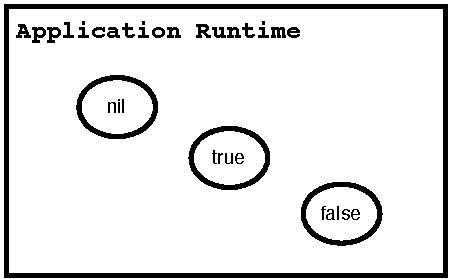
\includegraphics[width=.99\linewidth]{nil_creation}
\end{subfigure}
\caption{\textbf{Step 1: create the first well-known objects.} The \ct{nil}, \ct{true} and \ct{false} instances are created inside the application runtime.\label{fig:nil_creation}}
\end{figure}


\paragraph{\textbf{Step 2: Create basic language structures}}

The basic language structures are the minimal structure we need to create all the rest of the language elements~(cf. Figure \ref{fig:basic_structure_creation}). For example, creating a class requires the existence of a table of global objects to install the class, and a table of unique strings or symbols to have a unique identifier for it. We must create these basic structures from the very beginning, as the rest of the process rely on them.

\begin{figure}[ht]
\begin{subfigure}{.45\linewidth}
\begin{code}
globalTable := GlobalTable basicNew.
globalTable
    at: #GlobalTable
    put: globalTable.
    
SymbolTable initialize.
\end{code}
\end{subfigure}
\begin{subfigure}{.55\linewidth}
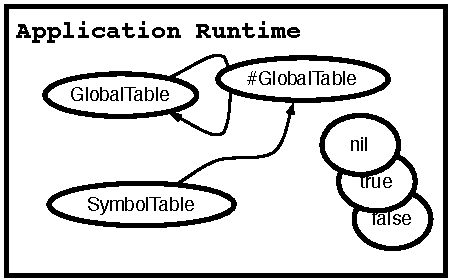
\includegraphics[width=.99\linewidth]{basic_structure_creation}
\end{subfigure}
\caption{\textbf{Step 2: Create basic language structures.} We create those structures that are required to create the rest of the language elements, such as the symbol and global tables. In the figure we can see that the global table references itself as a global and the symbol table references the \ct{GlobalTable} symbol.\label{fig:basic_structure_creation}}
\end{figure}

\paragraph{\textbf{Step 3: Create classes}}
We create the classes that the language definition requires in the language runtime~(cf. Figure \ref{fig:class_creation}). Pharo already includes a \emph{class builder} object that knows how classes should be created in the application runtime. The class builder validates that a class can be created, creates it and installs it inside the global table. The class builder encapsulates the complexity of class creation \eg first-class layouts, traits, first class instance variables. In this step we do not install a class' methods, since they can reference classes that are not created. We will create all methods at once in a next step once all classes are created.

\begin{figure}[ht]
\begin{subfigure}{.4\linewidth}
\begin{code}
nil subclass: #ProtoObject
    instanceVariableNames: ''.

ProtoObject
    subclass: #Object
    instanceVariableNames: ''.
\end{code}
\end{subfigure}
\begin{subfigure}{.6\linewidth}
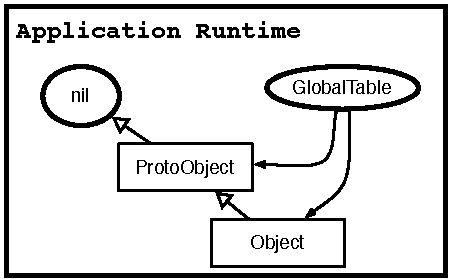
\includegraphics[width=.99\linewidth]{class_creation}
\end{subfigure}
\caption{\textbf{Step 3: Create classes.} Classes are created by the class builder and installed inside the global table. \label{fig:class_creation}}
\end{figure}

\paragraph{\textbf{Step 4: Installing methods}}

We compile~(if needed) and install each of the methods present in the language definition into their respective classes. Method literals are bound to their corresponding literals or global objects~(\eg classes).

\begin{figure}[ht]
\begin{subfigure}{.4\linewidth}
\begin{code}
ProtoObject >> isNil
   ^ false

UndefinedObject >> isNil
   ^ true
\end{code}
\end{subfigure}
\begin{subfigure}{.6\linewidth}
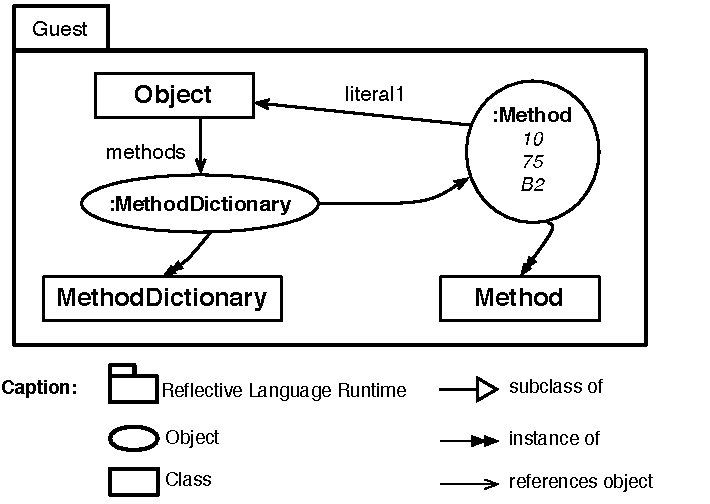
\includegraphics[width=.99\linewidth]{method_installation}
\end{subfigure}
\caption{\textbf{Step 4: Installing methods} The methods that appear in language definition are installed inside the application runtime. In this example the \ct{ProtoObject} and \ct{UndefinedObject} classes contain each an \ct{isNil} method.\label{fig:method_installation}}
\end{figure}


\paragraph{\textbf{Step 5: Initialization}}
%With all the classes and methods from the language specification installed, the structural part of the language is already set up. 
This last step consists in the execution of the class initializers. In Pharo, it consists into sending the message \ct{initialize} to those classes that require some kind of extra initialization. For example, at this point we create well-known float values~(\eg NaN or Infinity) and the thread machinery. At the end of this step, the language runtime is able to execute code by itself.

\begin{figure}[ht]
\begin{subfigure}{.4\linewidth}
\begin{code}
Float initialize.
Processor initialize.
\end{code}
\end{subfigure}
%\begin{subfigure}{.6\linewidth}
%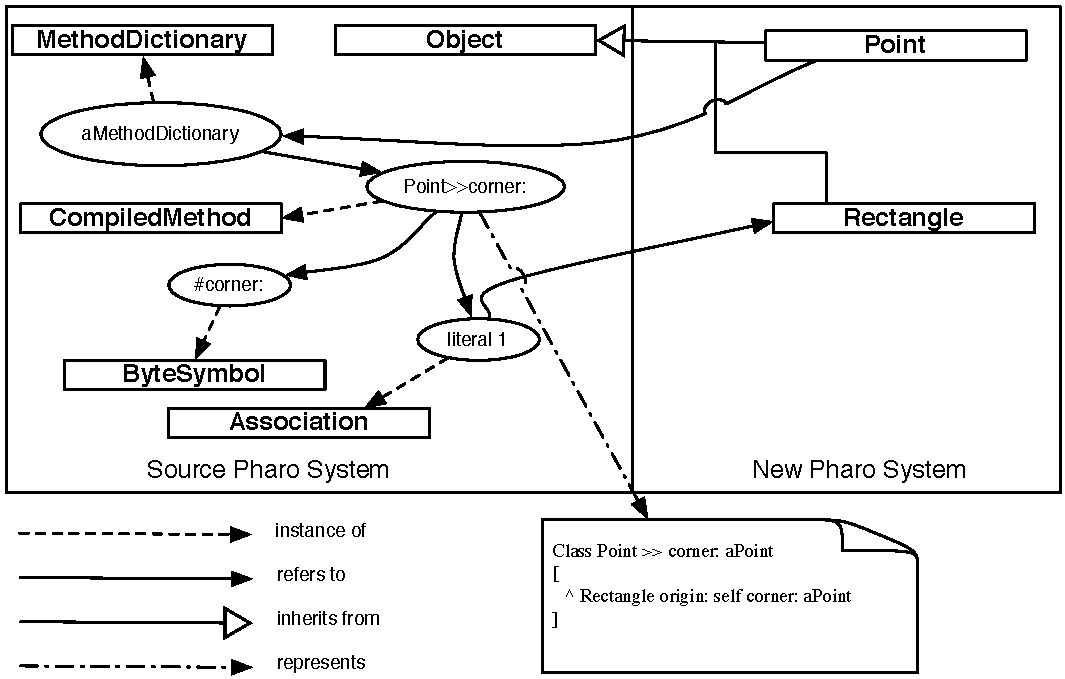
\includegraphics[width=.99\linewidth]{bootstrap_step4}
%\end{subfigure}
\caption{\textbf{Step 5: Initialization.} Class initializers are executed to setup the state of the class. In this example we initialize the \ct{Float} and \ct{ProcessScheduler} classes sending them the \ct{initialize} message.\label{fig:method_installation}}
\end{figure}


%\begin{figure}[ht]
%\begin{center}
%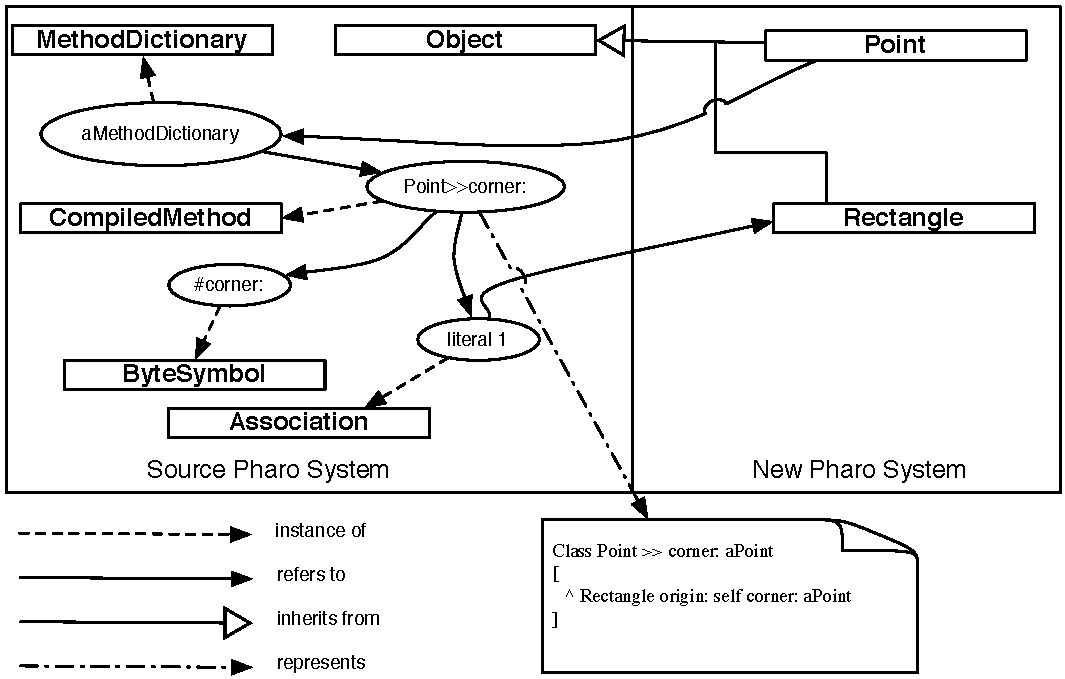
\includegraphics[width=0.6\linewidth]{bootstrap_step4}
%\caption{State of method literal resolution in the initial bootstrap.\label{fig:bootstrap_step4}}
%\end{center}
%\end{figure}


\section{Bootstrapping with \Vtt}\label{sec:bootstrapping_infrastructure}

To execute such a language definition, we developed a bootstrap infrastructure for an object-oriented language based on \Vtt~(Figure \ref{fig:bootstrapping_overview}). This infrastructure presents three explicit components that decouple the initialization of the language runtime from the \VM initialization so we can define different languages on top of the same \VM. Additionally we can modify the language runtime using the abstractions and tools of the high-level language.

\begin{figure}[ht]
\center
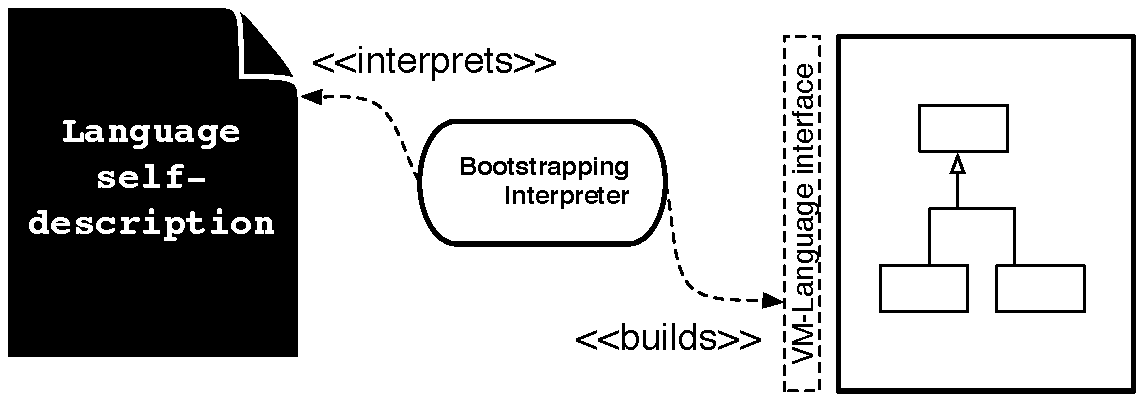
\includegraphics[width=.9\linewidth]{bootstrap_nutshell}
\caption{\textbf{Solution overview.} A bootstrapping interpreter uses the self-description in the language definition to build the language through the a clear \VM-language interface.\label{fig:bootstrapping_overview}}
\end{figure}

\begin{description}
\item[Language definition.] The code that defines the initialization of the language runtime is extracted and expressed in the same language it defines. This code is expressed as normal code of the language it defines. Thus, during the language initialization we can benefit from the abstractions and tools of the language we are defining. For our prototype implementation this self-description is a set of files.

\item[Virtualized Bootstrapped Language Runtime.] The bootstrapped language is initialized inside a virtualized runtime. This virtualized runtime is initially empty and the bootstrap process fills it with objects before it reaches the execution point. As such, we can use the object space clear \VM-language interface for its manipulation. This also serves the purpose of identifying what are the \VM and language concerns during language initialization to easily decouple them.

\item[Bootstrapping Hypervisor and Virtual Interpreter.] A \emph{bootstrapping hypervisor} contains an specialized virtual interpreter, the \emph{bootstrapping interpreter}. The bootstrapping interpreter is a specialized AST interpreter that can execute the code available in the language definition under the initial absence of classes and objects.
\end{description}

%The main limitation of our approach is the \VM execution model. Our solution exposes a clear but fixed \VM interface that introduces a common denominator for each of the languages we bootstrapped. The co-evolution of language runtime and \VM will be addressed in future work and is out of the scope of this thesis.

%\gp {should merge from here}
% ===========================================================================
%\section{Bootstrapping with \Vtt}\label{sec:bootstrapping_infrastructure}

%We implemented a bootstrapping infrastructure on \Vtt. In our solution, the bootstrapped language runtime will be created inside the virtualized runtime. The main component of the bootstrapping hypervisor is a \emph{bootstrapping interpreter}. The bootstrapping interpreter is a specialised AST interpreter that can execute the code available in the language definition under the initial absence of classes and objects~(Figure \ref{fig:objectSpaceOverview}).

%  on \emph{object spaces} and abstract interpretation~(cf. Figure \ref{fig:objectSpaceOverview}). An object space is a first class representation of an \emph{object runtime system}: it is an object that provide a high level API to manipulate an object runtime system. An object space \textbf{isolates} its represented object runtime system by using mirror objects~\cite{Brac04b}~(cf. Section \ref{sec:mirrors}). Abstract Syntax Tree~(AST) interpretation solves the remaining issues. First, the combination of object spaces and the AST interpreter allow multiple object runtime systems to co-exist and execute independently, overcoming the \textbf{unicity hyphotesis}~(cf. Section \ref{section:object_spaces} and Section \ref{sec:ast_interpreter}). Second, with AST interpretation we can execute code inside the guest language runtime, using the language specification as a source for both compilation and execution, \textbf{avoiding logic duplications}.
%
%In this section, we present how our solution supports the bootstrap process introduced in Section~\ref{sec:process} and solves our stated challenges. We provide the API of both our object spaces and mirror objects, and how our AST interpreter interacts with the object space infrastructure.

%\begin{figure}[ht]
%\center
%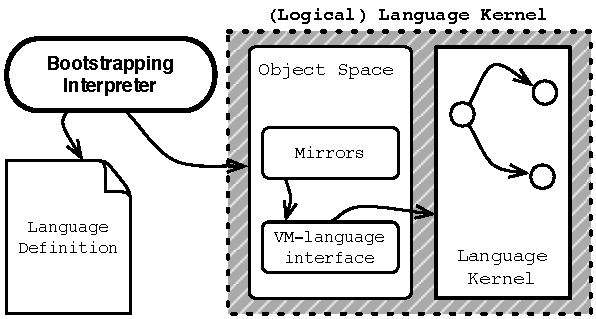
\includegraphics[width=.7\linewidth]{object_space_bootstrap_overview}
%\caption{\textbf{Solution overview in \Vtt.} The virtualized runtime will contain the bootstrapped language runtime. A \emph{bootstrapping interpreter} executes the language definition on the virtualized runtime using the object space interface.\label{fig:objectSpaceOverview}}
%\end{figure}

%To support the bootstrapping process in the time our bootstrapping infrastructure provides with measurement of change impact in a scenario where changes are common and bootstrapping must be performed continuously~(Section \ref{sec:continuous_bootstrapping}). We achieve this by integrating the bootstrapping process in a continuous integration environment. The bootstrapping interpreter traces the execution of the bootstrap and can provide the language developer with feedback about the impact of his/her changes.

%\subsection{Virtualized Runtime for Bootstrapping}\label{section:object_spaces}
%
%With \Vtt, an Object-Oriented language bootstrap generates the language elements~(objects, classes, methods, threads) inside a virtualized runtime. For bootstrapping purposes, this runtime is initially empty. 

\section{The Circular Language Definition}\label{sec:circular_definition}

The language definition describes the language we are bootstrapping. During the bootstrap process, the language runtime under construction traverses several stages until it is finished. When the bootstrap process starts, the language runtime is not yet able to execute code by itself \eg it cannot resolve the method lookup because the class hierarchy is not created. As we install packages or classes the language runtime reaches its \emph{execution point}, where it contains already the minimal set of elements it needs for execution. Later on, we can install reflective features into the language runtime to get it inside the \emph{reflective spectrum}. Figure \ref{fig:phases} illustrates the stages of a language runtime construction during the bootstrap process.

\begin{figure}[ht]
\center
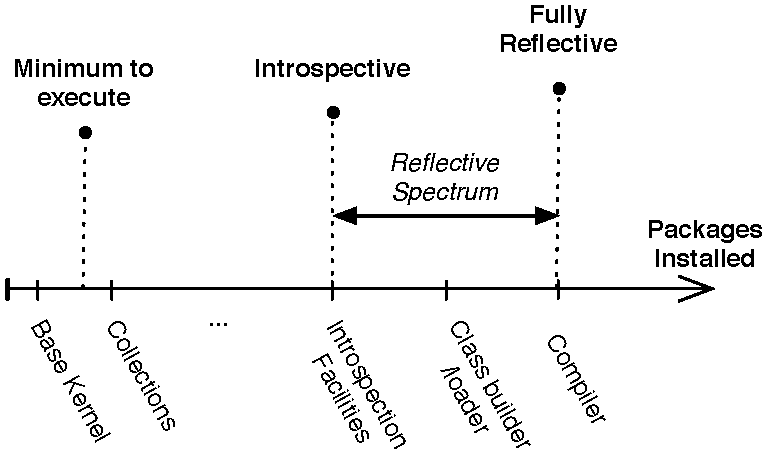
\includegraphics[width=.6\linewidth]{bootstrapping_phases}
\caption{\textbf{Bootstrap Phases.} Initially, a language runtime does not contain the minimal elements to execute code. As the bootstrap process installs elements, it reaches the point of execution where it can run autonomously. Later, when (if) reflective features are installed, it reaches the reflective spectrum.\label{fig:phases}}
\end{figure}

The \Vtt-based bootstrap process takes as input this language definition source code, parses it and reifies it as abstract syntax trees~(ASTs) of the language elements~(\eg classes and methods).
ASTs ease the manipulation of the language definition for its compilation, interpretation and extraction of information \eg we can easily extract variable and class names, superclasses, and know how to bind names during compilation. Figure \ref{fig:hazelSpecModel} illustrates our basic AST model. For example, a Class definition contains amongst others its name, its superclass, a list of the instance variables that it defines and the source code of its definition. A method definition contains its selector, a list of its statements and its full source code. For clarity of the figure, we don't include sub-method nodes such as statements, assignments or message sends in it.

\begin{figure}[ht]
\begin{center}
\includegraphics[width=\linewidth]{HazelSpecModel}
\caption{\textbf{Basic Bootstrap AST Model.}\label{fig:hazelSpecModel}}
\end{center}
\end{figure}

Inside a language definition we can identify two main sub-components, the language base-level entities and the language meta-level ones.

\subsection{Language base-level entities}

The language definition contains all those classes and methods that must be built and available to a program to run. We call these the base-level entities of a language definition. The base-level entities describe the basic class hierarchy of the language and basic objects such as strings or integers. The following code snippet illustrates how the base-elements of Pharo are described inside the language definition. Notice that this code snippet has the same responsibility than the Ruby \VM code we showed in the introduction of this chapter.

\begin{code}
nil subclass: #ProtoObject
    instanceVariableNames: ''.

ProtoObject >> isNil
    ^ false

ProtoObject subclass: #Object
    instanceVariableNames: ''.

Object subclass: #UndefinedObject
    instanceVariableNames: ''.
    
UndefinedObject >> isNil
    ^ true
    
Object variableByteSubclass: #String
    instanceVariableNames: ''.
    
...
\end{code}

\subsection{Language meta-level entities}
The language definition must also include elements that know how to create the base-level entities \eg a compiler or compiler interface~(to an external compiler). We need the language meta-level elements to create methods and classes during the bootstrap. Notice however that a language runtime must not necessarily include these elements at the end of the bootstrap. A bootstrap process that builds and introduces the meta-level elements inside the bootstrapped runtime is a \emph{reflective language runtime}.
A language that contains both introspection and full intercession facilities is a fully reflective language. A fully reflective language does not only have the minimal set of elements to run, but also the minimal to be autonomous: it can create/load classes and methods without any external component~(compiler, class builder, interpreter).

\begin{code}
Object subclass: #Compiler
    instanceVariableNames: ''.

Compiler >> compile: sourceCode in: aClass
    ...
    
Object subclass: #ClassBuilder
    instanceVariableNames: ''.
    
ClassBuilder >> buildClassNamed: aClassName withSuperclass: aSuperclass
    ...
\end{code}

The meta-level entities include in addition the code that defines the bootstrapping process \ie the steps that must be followed to create a coherent and well formed language runtime.

\begin{code}
nilObject := UndefinedObject basicNew.
trueObject := True basicNew.
falseObject := False basicNew.

globalTable := GlobalTable basicNew.
globalTable
    at: #GlobalTable
    put: globalTable.
    
SymbolTable initialize.

...
...
Float initialize.
ProcessScheduler initialize.
\end{code}

%\begin{figure}[ht]
%\center
%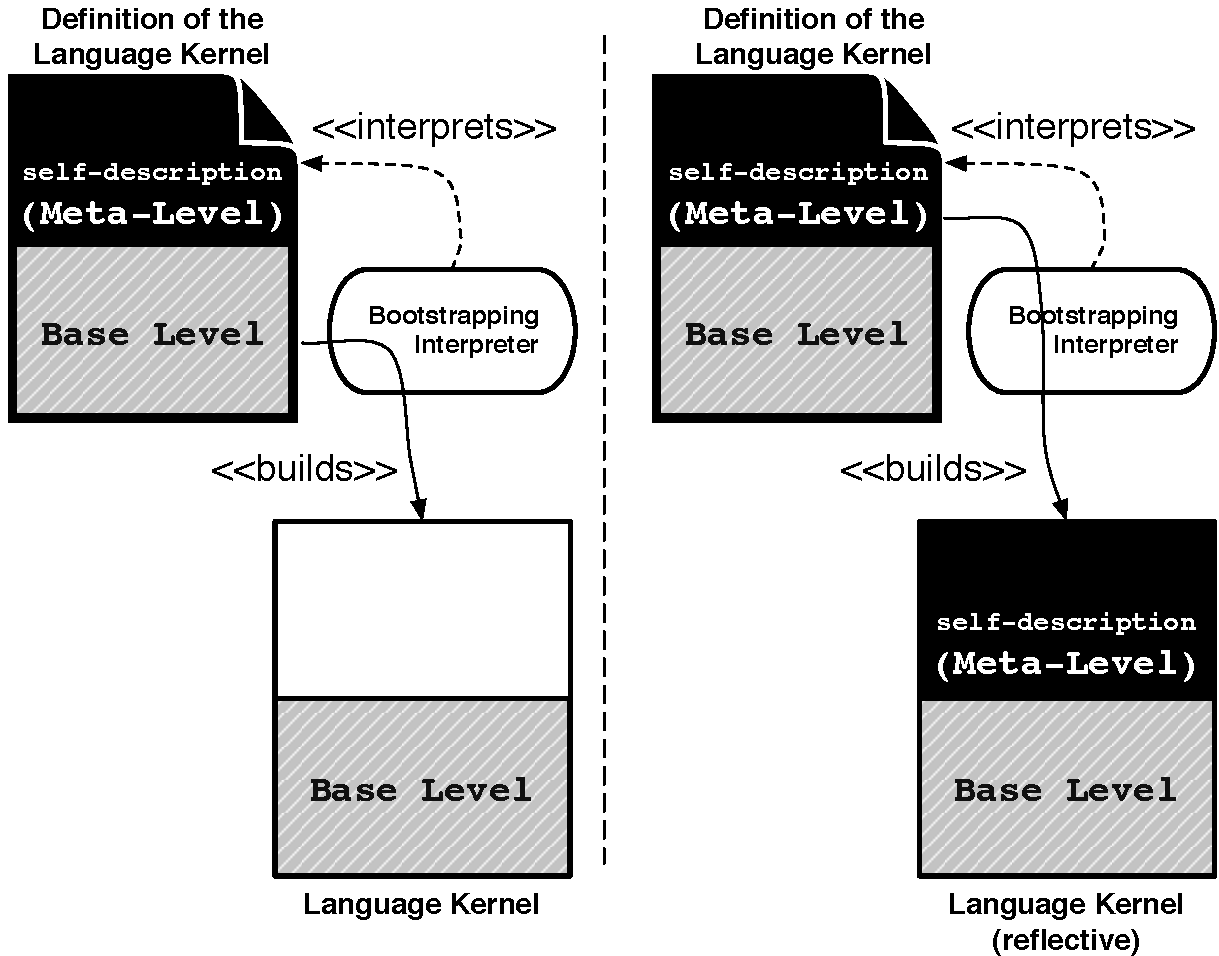
\includegraphics[width=.8\linewidth]{building_reflective_language}
%\caption{\textbf{The language definition in the bootstrap process.} The bootstrapping interpreter uses the meta-level of the language to build the base-level of the language~(left-side). Afterwards, it may inject the meta-level to make it a reflective language~(right-side).\label{fig:language_definition}}
%\end{figure}

%\begin{description}
%\item[The base-level language elements.]  We consider here those elements that are part of the \textbf{base-level}~(\eg basic language classes and libraries) of the language and also the ones in the \textbf{meta-level}~(\eg the reifications of the language runtime, a compiler interface, the class builder).
%
%\item[The meta-level language elements.]

%\section{The Bootstrapping Process}\label{sec:bootstrapping_process}
%The bootstrapping process requires a particular order as it sets up very interrelated dependencies amongst the language elements. In the case of reflective languages these dependencies are meta-circular~\cite{Stra14a,Chib96a,Maes87a,Smit84a}. The order and specifics to build the language must be described in the language definition. This process presents also which are the elements that will be introduced into the built language: it is here where we decide if the output language runtime will be reflective or not.
%
%\gp{extend in here}


\section{The Bootstrapping Interpreter}\label{sec:ast_interpreter}

The bootstrapping interpreter is a virtual code interpreter that interprets code expressed in the bootstrapped language. The bootstrap process uses the bootstrap interpreter to execute the language definition inside the virtualized runtime before it reaches the execution point. Its design present the following important properties that allow it to achieve this:

\begin{description}
\item[Alternative method lookup.] Before reaching the execution point, the class hierarchy of the language runtime is incomplete, or part of its methods are not yet installed. The bootstrapping interpreter implements an alternative method lookup mechanism to allow message sending before we reach the execution point: methods are looked up in the definition of the language instead of the hierarchy in the language runtime; a mapping is kept between classes created in the language runtime and their definitions in the language definition to know where the lookup should start.

\item[Automatic class stubs.] The bootstrapping interpreter does also solve most of the well known bootstrapping issues~(\eg how to create an instance before a class exists) in a generic way by using class stubs. When an inexistent class is needed during the bootstrap process, the interpreter creates an empty class to take its place respecting the \VM format for it. The interpreter will be able to create instances of this class and map it to its corresponding definition to perform the method lookup. This class cannot, however, initially perform reflective operations as it does not contain any reflective information. When the real class is created later on in the process, it replaces the stub. For this purpose, we extended the object space interface with one operation that allows the creation of an object whose class pointer is not initialized.

\begin{code}
objectSpace {
    mirror allocateObjectOfSize(int size);
}
\end{code}

\end{description}

\begin{figure}[!ht]
\center
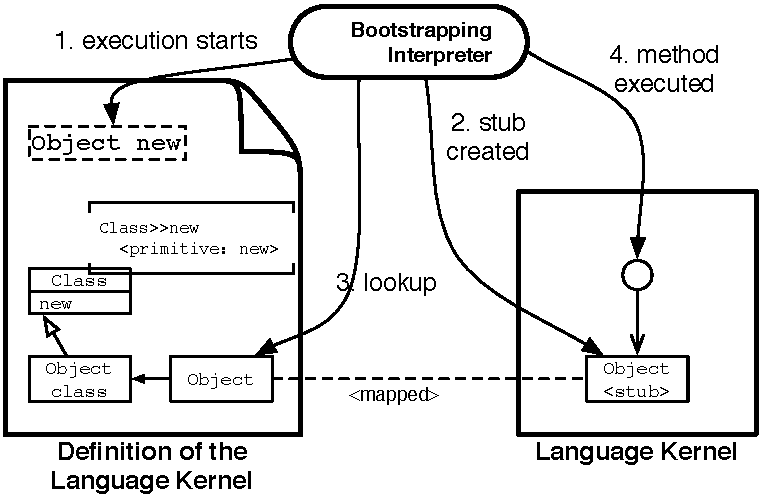
\includegraphics[width=.9\linewidth]{interpretation}
\caption{\textbf{The Bootstrapping interpreter in action.} A stub class is created for a non existent class. Each class is mapped to its description in the language definition. The lookup is then performed inside the language definition. Once the method is found, it is executed inside the language runtime.\label{fig:interpretation}}
\end{figure}

Figure \ref{fig:interpretation} illustrates with an example the behavior of the interpreter, particularly in the execution of the \ct{"Object new"} expression. First, if the class \ct{Object} does not exist, it create a stub \ct{Object} class and maps it to its corresponding definition in the language definition. To interpret the \ct{new} message, the interpreter performs the method lookup from the class of the object in the language definition. As the class from the language runtime and the language definition are mapped, the interpreter knows where to start the method lookup. The method is found in the \ct{Class} class and executed in the language runtime. As a result, an instance of the \ct{Object} class is created.

By using the bootstrapping interpreter, the language definition serves both as a source for compiling the code that will be part of the application runtime, and for the execution of the bootstrapping process itself. A change to the language definition will affect both and avoids major code and logic duplications between \VM, language, and language initialization. For example, Figure~\ref{code:logic_dup3} illustrates how we can use the interpreter to use the \ct{Dictionary} code from the language definition instead of the C function that is part of the \VM, as we shown in \chapref{state_modifying}.


\begin{figure}[ht]
\begin{code}
Bootstrap>>createDictionaryWith: n
    "Create a dictionary in the new language runtime"
    ^ interpreter
            execute: 'Dictionary new: size'
            binding: { 'size' -> n }.
\end{code}
\caption{\textbf{Avoiding logic duplications with the bootstrapping interpreter.} This example shows how the bootstrapping interpreter does not duplicate the logic of the \ct{Dictionary>>new:} method, but uses it instead.\label{code:logic_dup3}}
\end{figure}


\section{Continuous Bootstrapping}\label{sec:continuous_bootstrapping}

Building continuously a language runtime provides the language engineers with the same benefits of continuously building another application: automated integration and testing, quick and continuous feedback on the applied changes. This continuous feedback should give the language developer with the information and tools to resolve conflicts and problems: it should clearly show which was the \emph{impact} of such change in the process. A change introduced in the language impacts directly on the definition of the language~(Figure \ref{fig:impact}). The changed definition is used in turn by the bootstrap process to bootstrap the new version of the language runtime, thus the change has also an indirect impact on the bootstrapped language. 

\begin{figure}[ht]
\center
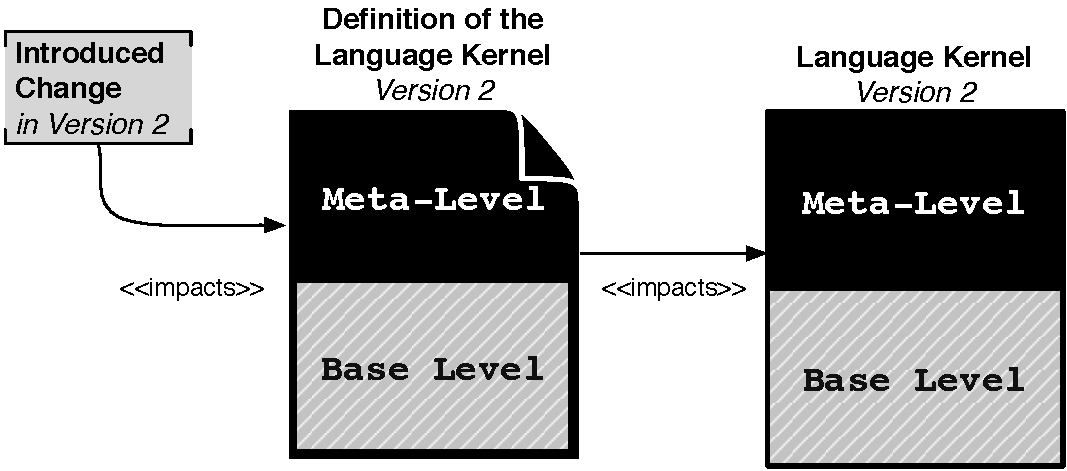
\includegraphics[width=0.7\linewidth]{impact}
\caption{\textbf{How a change impacts the bootstrap process.} A change in the language may impact directly the definition of the language, which in turn impacts the bootstrap process.\label{fig:impact}}
\end{figure}

However, not every change in the language definition may impact the bootstrap process: some code is only meant to be in the result of the bootstrap process but it is not used by the bootstrapping interpreter \eg changing the set of final classes introduced by the bootstrap does not alter the bootstrap process. To identify the impact of a change on the language in the bootstrap process we introduced as a second output of our bootstrapping interpreter an execution trace containing all the language elements that were used to bootstrap: any change on these elements may have an impact on the process. Then, to produce useful feedback for the changes made by a language developer, an \emph{impact resolver} measures the impact of a change on the bootstrap process by comparing the introduced change to the trace of previous bootstrap execution~(Figure \ref{fig:resolving_impact}).

Our bootstrapping infrastructure measures the impact by making a diff between the traced and changed language elements. In case a change breaks the bootstrap process, the language engineer has hints that helps him spotting the problem and act on it. We are working to obtain in the future more information through a smarter impact analysis.

\begin{figure}[ht]
\center
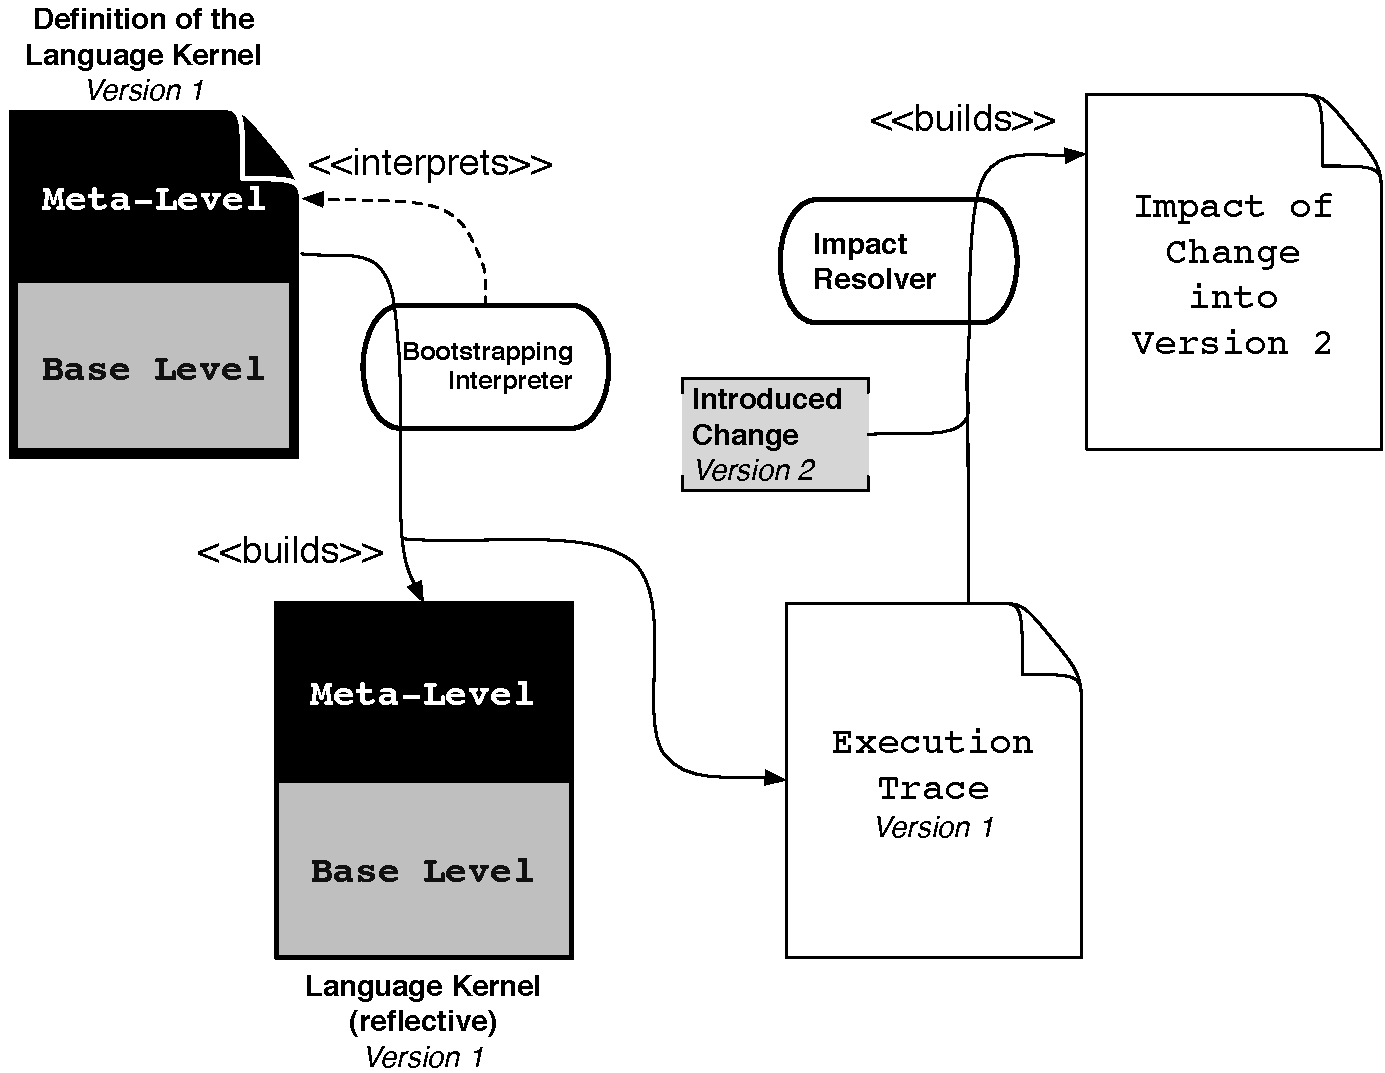
\includegraphics[width=.8\linewidth]{resolving_impact}
\caption{\textbf{How a change impacts the bootstrap process.} The bootstrap process execution is traced. An impact resolver decides if the introduced change will impact in the bootstrap process or not.\label{fig:resolving_impact}}
\end{figure}

\section{Conclusion and Summary}

Bootstrapping is commonly known by its usage on compiler building, where a compiler can compile itself.
It can be generalized to the introduction of any software system to its own building process.
A bootstrap process allows us to easily change this system as it is expressed in terms of itself, taking advantage of its abstractions and tools.

In this chapter we explored the bootstrap of an object-oriented language using \Vtt. By using \Vtt we can easily modify the bootstrapped language runtime even when it is empty. A virtual code interpreter, the bootstrapping interpreter, allows the execution of the language definition in an initially empty virtual runtime. On one side, it overrides the method lookup mechanism to look for method ASTs inside the language definition instead of inside the half-built bootstrapped language, avoiding duplications. On the other side it solves the bootstrapping issues by automatically creating class stubs and replacing them once we create and install the real classes.
%
%The main limitation of our approach is that we don't address the co-evolution of language and VM. A co-evolution implies changing not only language and VM but also their interface. We expect to address these issues in future work and see what the introduction of a metacircular-programming framework implies in this regard.

% ===========================================================================
\chapter{Bootstrapping Validation} \label{sec:bootstrapping_validation}
\minitoc
\introduction

In this chapter we present our results while bootstrapping four different case study languages.
To reuse the parsing infrastructure and the bootstrapping interpreter, the four bootstrapped languages share also the same syntax: a Smalltalk syntax. Although these similarities, each of the four language runtimes possess different model and semantics~(cf. Section \ref{sec:bootstrap_case_studies}):

\begin{description}
\item[Pharo.] Pharo is a fully-reflective language composed of classes and traits with first class slots and object layouts~\cite{Verw11a}.
\item[Metatalk with and without meta-level.] Metatalk~\cite{Papo11a} is a language that fully decomposes the meta-level from the base-level using mirrors, allowing us to bootstrap a reflective and a non-reflective version of Metatalk.
\item[Candle.] Candle is a partially reflective \ct{Smalltalk-80} based mini-kernel that includes introspection and some self-modification features.
\end{description}

Finally this chapter presents some measurements~(cf. Section \ref{sec:bootstrap_measurements}). To keep bootstrapping practical, we optimized the critical parts of the process for both the language user and the language engineer. On one side language users do not usually need to modify the language runtime but use it, independently of the language initialization process it provides. To suit this scenario we do not build the language runtime each time: we generate a snapshot with a cached version of it. On the other side we find language designers/engineers whose job is to change the language runtime. For them the bootstrap process must provide with an acceptable development cycle for activities like debugging. With this case in mind, we optimized the \emph{bootstrapping interpreter} with a dynamic compilation technique. Each of the measurements we present below were made on a 2.2 Ghz Intel Core i7 machine with 8 GB memory 1333 Mhz DDR3.

\section{Languages Used for Experimentation}\label{sec:bootstrap_case_studies}

Using \Vtt we bootstrapped four different object-oriented languages. These languages share two common properties: the execution model of its \VM and the Smalltalk syntax. They present different programming models for the developer \eg the absence of reflective features, their inclusion through mirrors, first-class variables and traits.
Figure \ref{fig:languages_spectrum} shows how these four languages are placed in the language spectrum. We explain more in detail these languages in the following subsections.% These results show that our process can produce different systems when fed with different specifications. The resulting bootstrapped systems are available at \url{http://ci.inria.fr/rmod/view/Oz/}.

\begin{figure}[ht]
\center
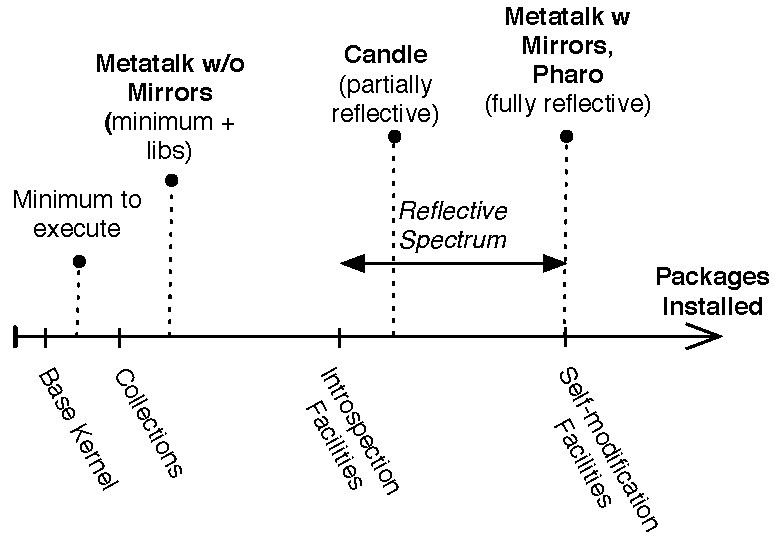
\includegraphics[width=.8\linewidth]{languages_by_reflectiveness}
\caption{\textbf{Bootstrapped Languages Spectrum.} How the languages we bootstrapped are placed in the reflective spectrum. In particular, Metatalk with and without its mirrors is in different extremes of the spectrum.\label{fig:languages_spectrum}}
\end{figure}


\subsection{Language I: Pharo}\label{sec:bootstrap_pharo}

Pharo~\cite{Blac09a} is an object-oriented reflective Smalltalk-inspired programming language. As it is a Smalltalk-80 inspired language, its class model includes implicit metaclasses: each class has its own metaclass, an instance of \ct{Metaclass}. Pharo also extends the execution model of its \VM with traits~\cite{Scha03a} and class extensions~(\ie the ability to add methods to a class that belongs to another package). Finally Pharo has first class instance variables (slots) structured in object layouts \cite{Verw11a}. Figure \ref{fig:pharo_simplified_model} shows how the elements of the language are related to each other; the diagram is not meant to reflect the actual class graph~(which is more complex) but the language concepts.

\begin{figure}[ht]
\center
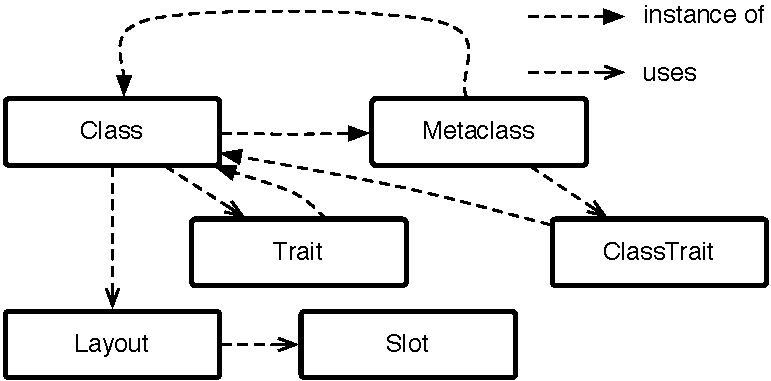
\includegraphics[width=.7\linewidth]{pharo_simplified_model}
\caption{\textbf{Simplified Pharo object model schema.} In Pharo each class has a metaclass. Metaclasses are defined circularly. Both classes and metaclasses makes use of trait objects to define part of their behavior. Classes also has layout that organises first class instance variables (slots). This schema does not represent the actual object graph, but a simplified picture.\label{fig:pharo_simplified_model}}
\end{figure}

Pharo is a fully-reflective language, placed at the end of the reflective spectrum. The Pharo language includes introspection in the kernel itself, and also self-modification stratified in three levels: object mutation facilities, a class builder and a compiler. The main challenge in Pharo is that the kernel itself of Pharo is defined by Traits: \eg the Trait class uses a Trait. First class slots are also part of the self-description of the language. This introduces new bootstrapping issues that must be resolved at bootstrapping time.

%Our resulting language runtime includes the packages defining Pharo's class model, traits, collections, the process scheduling library, the compiler and the class builder. The two latter allow the system to be extensible without external tools. With this selection we bootstrapped a language runtime that represents the 19\% of the original language runtime.
%The memory  the resulting bui language is 2MB, contrasting its 22MB original counterpart. \gp{remeasure it. Do we care about size?}

%Regarding its health, the boostrapped kernel can be tested using the SUnit testing framework.
%Unit tests of the kernel itself are loaded using the binary loader and run in the new system.
%Using this same mechanism, core packages like the compiler are able to be tested isolated from other libraries.

%A peculiarity of this system is that it is capable of bootstrapping a copy of itself.
%This is achieved by loading the binary packages of hazelnut and using it's own specification in the building process.
%Regarding the size of our obtained kernel, which is certainly not yet the minimal possible, our results shows that the design of the language runtime should be refined to create an even cleaner version.

\subsection{Languages II and III: Metatalk with and without Mirrors} \label{sec:bootstrap_metatalk}

Metatalk~\cite{Papo11a} is a reflective language where reflection is fully decomposed in explicit meta-objects, namely mirrors~\cite{Brac04b}. Metatalk makes the usage of reflection explicit: a program's execution takes place in the base-level of the language runtime, and it jumps to a meta-level when a mirror is used. Metatalk class model is simpler than Smalltalk's class model. It does not impose metaclasses. Instead, all classes are instances of the single \ct{Class} class. If there is a need for metaclasses~(to share behavior between classes), the developer can write its own explicit metaclasses~(Figure \ref{fig:metatalk_simplified_model}).

Metatalk mirrors decompose reflective behavior as well as the language meta-information \ie class' names, field order and names amongst others are part of its mirrors, and thus, they belong to the meta-level. When there is not a need for reflection, a Metatalk program can discard its meta-level with all the meta-information in it. The only staying meta-information is the one required by the \VMs execution model, such as the superclass relations, or the method selectors. This decomposition allows us to bootstrap Metatalk with or without its meta-level. This results in two different language runtimes: Metatalk base-level has no reflection at all, while Metatalk with both the base and the meta level is a fully-reflective language.

\begin{figure}[ht]
\center
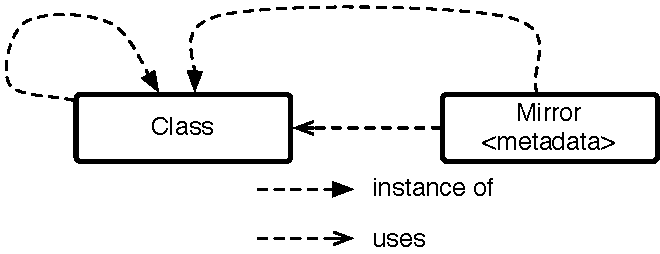
\includegraphics[width=.7\linewidth]{metatalk_simplified_model}
\caption{\textbf{Simplified Metatalk object model schema.} In Metatalk classes have no implicit metaclass. All classes share the same class. Mirrors are simple objects, thus instances of classes, that reflect on a class and contain their metadata. This schema does not represent the actual object graph, but a simplified picture.\label{fig:metatalk_simplified_model}}
\end{figure}

Metatalk's can be bootstrapped in two different ways. A non-reflective bootstrap initializes only the main classes of the language but does not create its meta-level. The non-reflective bootstrap does not contain mirrors. A second bootstrap creates a reflective Metatalk, which based on the latter one introduces the mirror instances with their corresponding metadata. We could bootstrap easily Metatalk in such a way due to the clear decomposition of its reflective elements. 

%%%%%%%%%%%%%%%%%%% Case of study and Results 2 %%%%%%%%%%%%%%%%%%%%
\subsection{Language IV: Candle} \label{sec:bootstrap_candle}

Candle is a Smalltalk-based language with a micro language runtime. Its class model includes implicit metaclasses as Smalltalk's and Pharo's one. However, Candle has no support for traits or slots~(Figure \ref{fig:candle_simplified_model}). We built Candle's language runtime by adapting MicroSqueak~\cite{Malo11a} to run on top of the Pharo \VM primitives. This micro language runtime was designed with the explicit goal of being the minimal distribution for the Squeak Smalltalk language.

\begin{figure}[ht]
\center
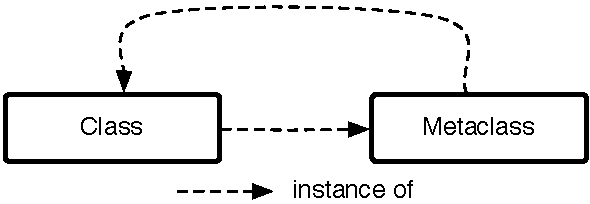
\includegraphics[width=.6\linewidth]{candle_simplified_model}
\caption{\textbf{Simplified Candle object model schema.} Candle follows a more traditional Smalltalk-80 model. In Candle each class has a metaclass. Metaclasses are defined circularly. There are no traits. This schema does not represent the actual object graph, but a simplified picture.\label{fig:candle_simplified_model}}
\end{figure}


Candle is a partially reflective language defined by a total of 49 classes and a reduced set of methods. Candle includes a minimal core of the language, a basic collection library and basic file IO support. It also provides with object introspection and mutation facilities. It does not include, however, a class builder or compiler to extend itself.%A bootstrapped Candle kernel presents a memory footprint of 80KB, with potential applications in embedded devices with little available memory.\gp{remeasure it. Do we care about size?}

\section{Measurements}\label{sec:bootstrap_measurements}

In this section we present the benchmarks we did to measure the bootstrap time of each of our four languages using our standard infrastructure. Table \ref{tb:measurements} shows the time to bootstrap each of the four languages using an unoptimized AST interpreter. This time comprehends the entire bootstrap process: from parsing the code in the language definition to its complete setup. We executed each of these benchmarks 10 times. The results table puts also the results in context: it presents how many code entities~(classes, traits, mirrors) and methods are built for each language. Notice that the bootstrapping time depends on the amount of elements it builds and also on their complexity. For example, creating a class in Pharo involves a biggest graph of objects than in the other two languages (because of the introduction of traits and class layouts). Section \ref{sec:optimisations} introduces two optimizations we did based on these measurements, that focus on the startup time and the development cycle of the bootstrap. 

 \begin{table}[ht]
 \small
 	\centering
 	\begin{tabular}{lcc}
			\toprule
			\textbf{Language}
			& \xspace\textbf{Code entities / Methods}\xspace
			& \xspace\textbf{Bootstrap time}\\
		\toprule
		Pharo & 626* / 6812 & 2h30m +/-10m \\\midrule
		Candle & 100* / 875 & 87s +/-8s \\\midrule
		Metatalk w/o mirrors & 25 / 114 & 0.957s +/-0.112s \\\midrule
		Metatalk reflective & 58* / 166 & 13.697s +/-0.061s \\\bottomrule
 	\end{tabular}
		\vspace*{0.2cm}
 	\caption{\small\textbf{Building Benchmarks.} Comparing the execution time of the bootstrapped languages using AST interpretation. (*) Pharo and Candle have implicit metaclasses, meaning that for each created class, an associated metaclass is created even if not necessary. Metatalk introduces a mirror object for each of the classes in the language.\label{tb:measurements}}
 \end{table}

We can observe from our measurements that bootstrapping Metatalk takes in average 1 second if no mirrors are created and 13 seconds if we include reflection in it. Candle bootstrap is slower, in the order of 1 minute and a half, mainly because it contains eight times more methods than the Metatalk. We can see that a plain AST-based bootstrapping interpreter has a a bigger impact in the bootstrap time if the language contains complex structures to initialize.  Indeed, creating a Pharo class using the AST interpreter is an operation that takes in average 17 seconds, because each class contains a reification of its memory layout and slots~\cite{Verw11a}. This problem is aggravated by the amount of classes and methods in this language definition.

Particularly about bootstrapping Pharo, a lack of modularity of the language impacts in the amount of code elements we have to build. Pharo's language runtime is historically a monolithic system which precludes us to build a minimal system. In fact, the Pharo language runtime we are bootstrapping represents a subset of the full Pharo language as it is distributed. This subset is planned to be the starting point for a more modular Pharo distribution.

\section{Optimizations}\label{sec:optimisations}

To be useful in practice, we understand that the bootstrap process should have the following two properties: (a) be fast enough to provide a good feedback loop and allow debugging to the language engineer and (b) provide a short startup time for the language users. Optimizing a bootstrap process is indeed a challenge since we cannot optimize it statically by fixing the meta-level semantics, as changing them is the main purpose of the bootstrap. In the following sections we show how snapshotting and dynamic compilation aid in these two optimization scenarios. 

\subsection*{Enhancing Bootstrap Time: Dynamic Compilation}
Since the main purpose of the bootstrap process is to easily change the meta-level semantics and structure of the language entities we cannot fix them statically to optimize them. In exchange, we chose to optimize the interpretation cycle using a dynamic compiler. The dynamic compiler compiles the interpreted code on demand. This compiled code is cached and executed directly on the \VM bypassing the interpretation step in following executions. We implemented dynamic compilation to optimize Pharo as it presents the worse of our results~(cf. Table \ref{tb:dynamic_compilation}). We reduced the total bootstrap time by a factor of 2.85. Additionally, we observed a mayor improvement on class creation, where the time improves from 17 to less than half a second. Class creation has a great impact on the Pharo's total bootstrap time, as it is executed 313 times. Contrastingly, the initial setup of the language structures~(\eg the symbol and character table, the initial threads) is executed only once where the cost of our dynamic compilation implementation increases the execution time. Notice that the current implementation does not optimize method compilation nor parsing, meaning there is still a room for improvement.

 \begin{table}[ht]
 \small
 	\centering
 	\begin{tabular}{lccc}
			\toprule
			\textbf{Case}
 			& \textbf{AST Interpretation}
			& \textbf{Dynamic Compilation}
			& \textbf{Gain}\\
			&&& \textbf{Factor}\\
		\toprule
		Total Bootstrap & 2h30m +/-10m & 53m +/-3.65m & 2.85x\\\midrule
 		Initial Setup& 4m8s +/-9s & 5m20s +/-40s & 0.77x\\\midrule
		Creation of one class & 17s +/-1s & 0.432s +/-0.189s & 39.85x\\\bottomrule
 	\end{tabular}
	\vspace*{0.2cm}
 	\caption{\small\textbf{Comparison of bootstrap time in absence and presence of dynamic compilation.}\label{tb:dynamic_compilation}}
 \end{table}

\subsection*{Optimizing Startup Time: Snapshotting.}
The user of a programming language is concerned about writing applications that run on this programming language instead of changing the programming language. From a user perspective the initialization of the language is transparent within the startup of an application. It should be however fast and ensure always the same state.
The language initialization present in production \VMs provides both properties. Bootstrapping, in the sense of this paper, turns this process slower due to the interpretation step.

For language users, we overcome this slow-down by \emph{caching} the result of our bootstrap process in a snapshot, as it is used in Smalltalk and Lisp\gp{cite}. Thus, we bootstrap a language runtime only when we change it, and otherwise we load the cached version. Caching keeps both properties of application startup: it guarantees the same state and it is faster. Table \ref{tb:startup} shows a comparison in the startup time of our \VM loading Pharo, Metatalk and Candle using snapshots, in contrast with Ruby. We measured the startup times by running each of them 10 times and making an average. From the results, we observe our startup time is bigger than ruby's but still reasonable, under the half of a second.

 \begin{table}[ht]
 \small
 	\centering
 	\begin{tabular}{lc}
			\toprule
			\textbf{Language}
 			& \textbf{Startup time}\\
		\toprule
		Ruby &  64ms +/-7.1\\\midrule
		Pharo & 280.8ms +/-3.4\\\midrule
		Candle & 186ms +/-7.6\\\midrule
		Metatalk w/o mirrors &202ms +/-13\\\midrule
		Metatalk reflective &205ms +/-11\\\bottomrule
 	\end{tabular}
	\vspace*{0.2cm}
 	\caption{\small\textbf{Startup time in perspective.} Comparing the startup time of a ruby application with the same in Pharo or Candle using a snapshot.\label{tb:startup}}
 \end{table}

Implementation-wise, the snapshot we used is a memory dump of the \VM heap. This heap will contain all the objects, classes and methods we created during the bootstrap. At load time, the memory dump is restored into memory and the \VM internals are re-configured to use this heap using the \VM setup interface. This idea is the same used by languages such as Smalltalk, Lisp, Javascript in V8 or the JikesRVM~\cite{Alpe00a}. Loading a binary image is as fast as reading the file and putting its contents inside the \VM's heap.

% ===========================================================================
\section{Conclusion and Summary}

%This chapter presents a bootstrap process for object-oriented languages based on \Vtt. Bootstrapping is a process for generating an application runtime from an explicit description of it. \Vtt supports this generation by providing hosting the runtime under construction inside a virtualized environment. Then, an object space's API exposes the operations needed for such creation.


We bootstrapped four different languages that have key differences in their meta-models: the core of the Pharo language is defined by traits, class layouts and first-class slots, Candle is a minimal Smalltalk with implicit metaclasses, finally Metatalk decomposes reflection from the base level and stores meta information in the meta level of the language. By using \Vtt these four languages run on top of the same Pharo Virtual Machine.

Then, we showed also that bootstrapping can be applied in a real environment. A fast startup can be achieved by caching the language runtime and a fast development cycle can be obtained by optimizing the bootstrapping interpreter through dynamic compilation.
% =============================================================================
\input{chapter-footer.tex}